\documentclass[a4paper,10pt]{article}
\usepackage{graphicx}
\usepackage[english]{babel}
\usepackage{geometry}           
\geometry{letterpaper}                   
\usepackage{graphicx}
\usepackage{amsmath}
\usepackage{amssymb}
\usepackage{wrapfig}
\usepackage[section]{placeins}
\usepackage{fontspec,xltxtra,xunicode}
\title{Three-Dimensional Vizualization and Animation\\Technical Report - Assignment II.}
\author{
  Marfeychuk, Mykhaylo\\
  \texttt{ist194039}
  \and
  Skalický, Matyáš\\
  \texttt{ist194904}
}

\date{} % 31.10.2019

\begin{document}
\maketitle

%\begin{figure}[!htb]
%	\centering
% 	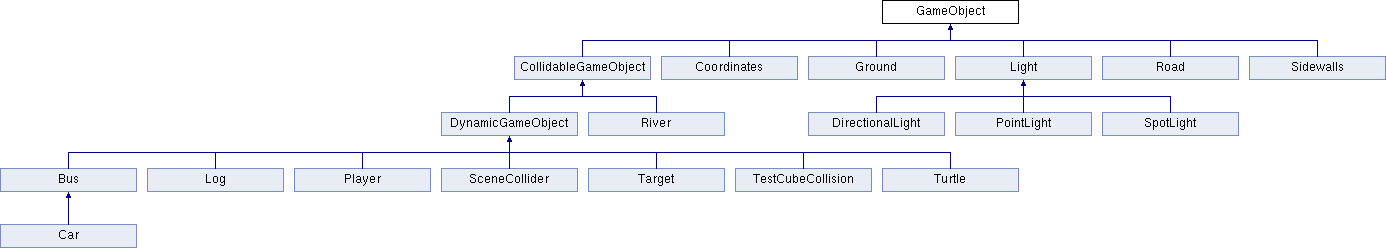
\includegraphics[width=\linewidth]{images/image1.png}
%  	\caption{Objects which inherit from the GameObject class.}
%\end{figure}

\section{Stencil test}
The stencil test is used in two parts of the game. First, it is used in the screen space in order to add black shadows to the game viewport. Original intention was to place the HUD to this space, however the hud is still missing and sadly was not implemented since the first task.

\section{Blending mechanism}
Todo

\section{Billboards}
To add the feeling of immersive game scenery, we utilized the tree textures and parts of the laboratory example code from the excercise. We utilize the cylindrical billboarding in order to restrict the trees from rotating away from the ground. This is done using a camera position alignment opposed to the reseting the rotation in the ModelView matrix. This is more computationally intensive, however allows us to easily limit the rotation around the ``up'' axis.

\section{Particle system}
The particle system implemented in the game is to animate the dirt flying away when the player lands on the ground. We use the player's velocity to set the horizontal speed of the particles, the upward and sideways force is slightly randomized. At each physics update, we multiply the particle's speed by deltaTime in order to preserve the physics even with different frame rendering times. We apply a downward force at each particle each physics step to simulate the gravity.

\section{Fog effect}
In order to implement the fog effect, we first calculate the vertex position in the vertex shader and pass it into the fragment shader. To get the shadow intensity, we calculate the distance from the camera to the fragment. Based on the distance, we blend the fog color into the resulting fragment color. The user can toggle the fog effect by pressing the ``f'' button.

\section{Lens flare effect}
Todo

\section{Planar shadows}
Todo

\section{Planar reflections}
Todo

\section{Bump mapping}
Todo

\section*{Conclusion}
We have continued working on the game as presented in the assignment 1. We have enhanced it with the required features as well as many graphical and playable improvements. For example, the movement of the player now resembles jumping. Also, we have improved the models (most notably the turtle model) and some of the textures.

Sadly, one of the members of our group agreed to do his part of work, but has failed to deliver any results. This is only a consequence of him not providing any of the work during the first task. Based on his performance, we have concluded that he should be evicted from our group as he only uses the results of our work without creating anything.

Mykhaylo Marfeychuk has also contributed very little to the work before the official deadline as he forgot about the deadline. He has, however, finished the work needed during the week before this report was submitted.
\end{document}  